\section{Posterior Distributions}
The posterior distribution is used to estimate a variety of model parameters of interest, such as the mean, the median, the mode, and so forth. \par It is possible to construct \textbf{credible intervals/regions} directly from the posterior (in contrast to the ``confidence'' intervals of frequentist inference). 
\newl Given a posterior distribution on a parameter $\theta$, a $1-\alpha$ credible interval $[L,U]$ is an interval such that
$$ P(L \leq \theta \leq U|D)\geq 1-\alpha.$$
Because the posterior is a full distribution on the parameters, it is possible to make all sorts of probabilistic statements about their values, such as:
\begin{itemize}[noitemsep]
	\item ``I am 95\% sure that the true parameter value is bigger than 0.5.''
	\item There is a 50\% chance that  $\theta_{1}$ is larger than $\theta_{2}$  .
  \item etc.
\end{itemize}
The best approach is to build the credible interval of $\theta$-values using the \textbf{highest density interval} (HDI), i.e.\@ to define a region $C_k$ in the parameter space with 
$$ C_k = \left\{\theta: P(\theta|D)\geq k\right\},$$
where $k$ is the largest number such that
$$ \int_{C_k} P(\theta|D)\, d\theta = 1-\alpha.$$
This typically has the effect of finding the smallest (in measure) region $C_k$ meeting the criterion.\par The value $k$ can be thought of the height of a horizontal line (or hyperplane, in the case of multivariate posteriors) overlaid on the  posterior and whose intersection(s) with the latter define a region over which the integral of the posterior is $1-\alpha$. In most cases, the value $k$ can be found numerically. 

\begin{Example}
\textit{HDIs, elections, and iterative data collection.} It is an election year and you are interested in knowing whether the general population prefers candidate $A$ or candidate $B$. A recently published poll states that of 400 randomly sampled people, 232 preferred candidate $A$, while the remainder preferred candidate $B$.
\begin{enumerate}[noitemsep,label=(\alph*)]
\item Suppose that before the poll was published, your prior belief was that the overall preference follows a uniform distribution. What is the 95\% HDI on your belief after learning of the poll result?  
\newl 
\textbf{Solution}: let preference for candidate $A$ be denoted by 1, and preference for candidate $B$ by 0. We can use the R function \texttt{BernBeta()} as in Example~\ref{ex4}. At the prompt, type
\newl \footnotesize \texttt{> post=BernBeta(c(1,1),c(rep(1,232),rep(0,168))) }\normalsize\newl
 yielding a posterior with a 95\% HDI from 0.531 to 0.628 for probability of candidate $A$.
\begin{center}		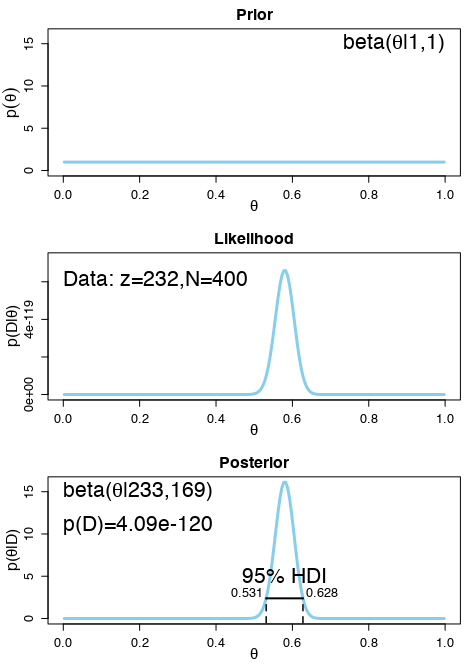
\includegraphics[width=\linewidth]{Images/example8a}
\end{center}
\item  Based on the poll, is it credible to believe that the population is equally divided in its preferences among candidates? \newl \textbf{Solution:} the HDI from Part (a) shows that $\theta=0.5$ is not among the credible values, hence it is not credible to believe that the population is equally divided in its preferences (at the 95\%) level.
\item You want to conduct a follow-up poll to narrow down your estimate of the population's preference. In the follow-up poll, you randomly sample 100 people and find that 57 prefer candidate $A$. Assuming that the opinion of people have have not changed between polls, what is the 95\% HDI on the posterior? \newl \textbf{Solution:} 
at the prompt, type \newl \footnotesize \texttt{
> post=BernBeta(post,c(rep(1,57),rep(0,43)))}\normalsize \newl
yields the figure on the next page. The 95\% HDI is a bit narrower for preference for candidate $A$ is a bit nanarrower, from 0.534 to 0.621.
\begin{center}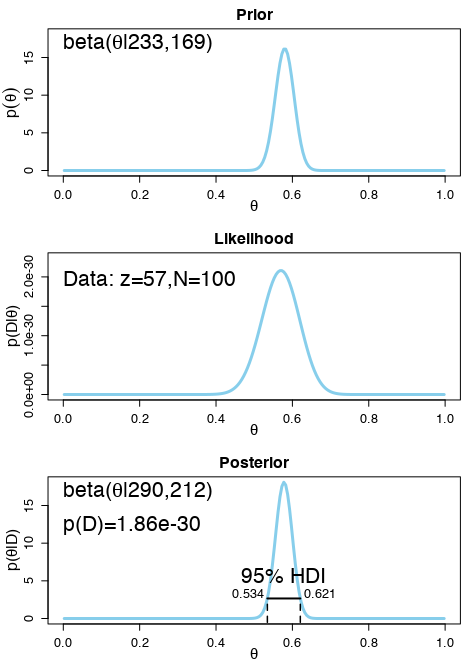
\includegraphics[width=\linewidth]{Images/example8b.png}\end{center}
 \item Based on the follow-up poll, is it credible to believe that the population is equally divided in its preferences among candidates?\newl\textbf{Solution:} the HDI from (c) excludes $\theta=0.5$; both the follow-up poll and the original poll suggest that the population is not equally divided (and actually prefers candidate $A$).
\end{enumerate}
\end{Example}
\subsection{Markov Chain Monte Carlo (MCMC) Methods}
The true power of Bayesian inference is most keenly felt when the model specifications lead to a posteriors that cannot be manipulated analytically; in that case, it is usually possible to recreate a synthetic (or \textbf{simulated}) set of values that share the properties with a given posterior. Such processes are known as \textbf{Monte Carlo simulations}.    
\newl A \textbf{Markov chain} is an ordered, indexed set of random variables (a stochastic process) in which the values of the quantities at a given state depends probabilistically only on the values of the quantities at the preceding state. \textbf{Markov chain Monte Carlo} (MCMC) methods are a class of algorithms for sampling from a probability distribution based on the construction of a Markov chain with the desired distribution as its equilibrium distribution.  The state of the chain after a number of steps is then used as a sample of the desired distribution. The quality of the sample improves as a function of the number of steps. \newl 
MCMC techniques are often applied to solve integration and optimization problems in large-dimensional spaces. These two types of problem play a fundamental role in machine learning, physics, statistics, econometrics and decision analysis. For instance, given variables $\theta\in\Theta$ and data~$D$, the following (typically intractable) integration problems are central to Bayesian inference:
\begin{itemize}
	\item \textbf{normalisation} -- in order to obtain the posterior $P(\theta | D)$ given the prior $P(\theta)$ and likelihood $P(D|\theta)$, the normalizing (denominator) factor in Bayes' theorem needs to be computed
	$$P( \theta | D ) = \frac{P(\theta)  P(D|\theta)}{\int P(D|\theta) P(\theta) d\theta}. $$

  \item \textbf{marginalisation} -- given the joint posterior of $(\theta,x)$, we may often be interested in the marginal posterior 
	$$ P(\theta|D) = \int P(\theta,x|D) dx.$$
	
	\item \textbf{expectation} -- the final objective of the analysis is often to obtain summary statistics of the form
	       $$ E(f(\theta)) = \int_{\Theta} f(\theta) P(\theta|D) d\theta $$
				for some function of interest (i.e. $f(\theta) =\theta$ (mean), or $f(\theta) = (\theta-E(\theta))^{2}$ (variance)). 
\end{itemize}

\subsubsection*{The Metropolis-Hastings (MH) Algorithm}
The Metropolis-Hastings (MH) algoirthm is a specific type of Monte Carlo process; it is likely among the ten algorithms that have had the greatest influence on the development and practice of science and engineering in recent times. \par MH generates a random walk (that is, it generates a succession of posterior samples) in such a way that each step in the walk is \textbf{completely independent} of the preceding steps; the decision to reject or accept the proposed step is also independent of the walk's history. \newl Any process for which the current step is independent (forgetful) of the previous states, namely
$$P(X_{n+1}=x|X_1=x_1,\ldots,X_n=x_n)=P(X_{n+1}=x|X_n=x_n)$$ for all $n$, $X_j$ and $x_j$, $j=1,\ldots, n$, is called a \textbf{(first order) Markov process}, and a succession of such steps is a \textbf{(first order) Markov chain}.  \newl MH uses a candidate or proposal distribution for the posterior, say q($\cdot$, $\theta$), where $\theta$ is a vector of parameters that is fixed by the user-called tuning parameters; MH then constructs a Markov Chain by proposing a value for $\theta$ from this candidate distribution, and then either accepting or rejecting this value (with a certain probability). \newpage\noindent Theoretically the proposal distributions can be nearly any distribution, but in practice it is recommended that (really) simple ones be selected: a normal if the parameter of interest can be any real number (e.g. $\mu$), or a log-normal if it has positive support (e.g. $\sigma^{2}$), say. \newl
The \textbf{Metropolis-Hastings} (MH) algorithm simulates samples from a probability distribution by making use of the full joint density function and (independent) proposal distributions for each of the variables of interest. 

\begin{algorithm}
\SetAlgoLined
\caption{Metropolis-Hastings Algorithm}
\text{Initialize } $x^{(0)}\sim q(x)$ \\
\For{$i=1,2,\cdots$} {
\it{Propose: } $x^* \sim q(x^{(i)}| x^{(i-1)})$ \\
\it{Acceptance Probability: } 
$$ \alpha(x^*|x^{(i-1)}) = min\left\{1, \frac{q(x^{(i-1)}|x^*)\pi(x^*)}{q(x^*|x^{(i-1)})\pi(x^{(i-1)})}\right\}$$

$u \sim \text{U}(0,1)$ \\
\uIf{$u<\alpha$}
{\it{Accept the proposal: }$x^{(i)}\gets x^*$ }
\Else
{\it{Reject the proposal: }$x^{(i)}\gets x^{(i-1)}$}
}
\label{algorithmMH}
\end{algorithm}
\noindent The first step is to \textbf{initialize the sample value} for each random variable (often obtained by sampling from the variable's prior distribution). The main loop of Algorithm 1 consists of three components: 
\begin{itemize}[noitemsep]
	\item \textbf{generate a candidate sample} $x^*$ from the proposal distribution $q(x^{(i)}| x^{(i-1)})$;
	\item \textbf{compute the acceptance probability} via the acceptance function $\alpha(x^*|x^{(i-1)})$ based on the proposal distribution and the full joint density $\pi(\cdot)$;
	\item \textbf{accept the candidate sample} with probability $\alpha$, the acceptance probability, or \textbf{reject it} otherwise. 
\end{itemize}

\begin{Example} \textit{The MH algorithm and simple linear regression.} The \textbf{test data} for this example is genreated using the following code. 
\begin{lstlisting}
t.A <- 10 # true slope
t.B <- 0 # true intercept
t.sd <- 20 # true noise
s.Size <- 50 # sample size
# create independent x-values 
x <- (-(s.Size-1)/2):((s.Size-1)/2)
# create dependent values according to ax + b + N(0,sd)
y <-  t.A * x + t.B + rnorm(n=s.Size,mean=0,sd=t.sd)
plot(x,y, main="Test Data")
\end{lstlisting}
\noindent Notice that the $x$ values are balanced around zero to "de-correlate" slope and intercept.  The result should look like the chart below.  
\begin{center}
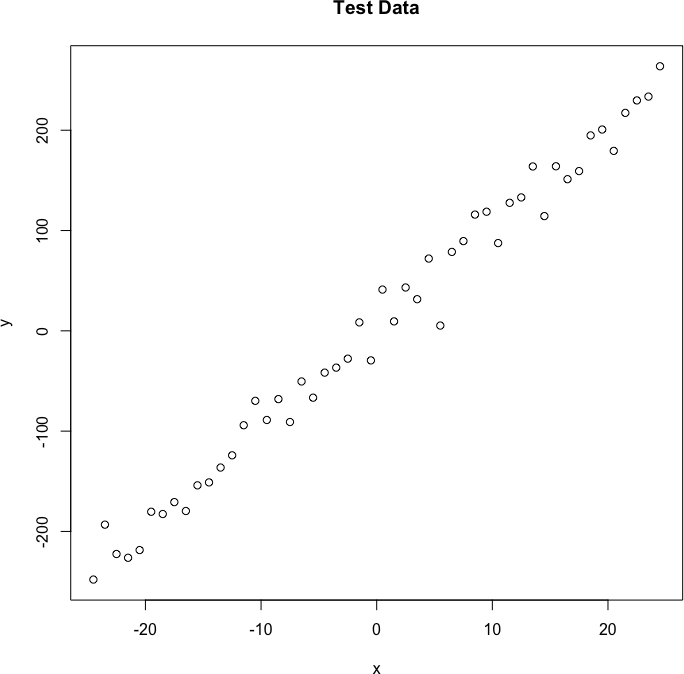
\includegraphics[width=\linewidth]{Images/example9a.png}
\end{center}

 
\item \textbf{Defining the statistical model.} The next step is to specify the statistical model. We already know that the data was created with a linear relationship $y = ax + b$ together with a  normal error model $N(0,sd)$ with standard deviation $sd$, so we might as well use the same model for the fit and see if we can retrieve our original parameter values. Note however that, in general, the generating model is unknown.


\item \textbf{Deriving the likelihood function from the model}. A linear model of the form $y = ax + b + N(0,sd)$ takes the parameters $(a, b, sd)$ as inputs. The output should be the probability of obtaining the test data under this model: in this case, we only need to calculate the difference between the predictions $y = ax + b$ and the observed $y$, and then look up the probability (using \texttt{dnorm}) for such deviations to occur.

\begin{lstlisting}
likehd <- function(param){
    a = param[1]
    b = param[2]
    sd = param[3]
    pred = a*x + b
    singlelikelihoods = dnorm(y, mean = pred, sd = sd, log = T)
    sumll = sum(singlelikelihoods)
    return(sumll) }
# Example: plot the likelihood profile of the slope a
s.values <- function(x){return(likehd(c(x, t.B, t.sd)))}
s.likehds <- lapply(seq(1/2*t.A, 3/2*t.A, by=.05), s.values )
plot(seq(1/2*t.A, 3/2*t.A, by=.05), s.likehds , type="l", xlab = "values of slope parameter a", ylab = "Log likelihood")
\end{lstlisting}
\noindent As an illustration, the last lines of the code plot the Likelihood for a range of parameter values of the slope parameter $a$. The result should look like the image below. 
\begin{center}
		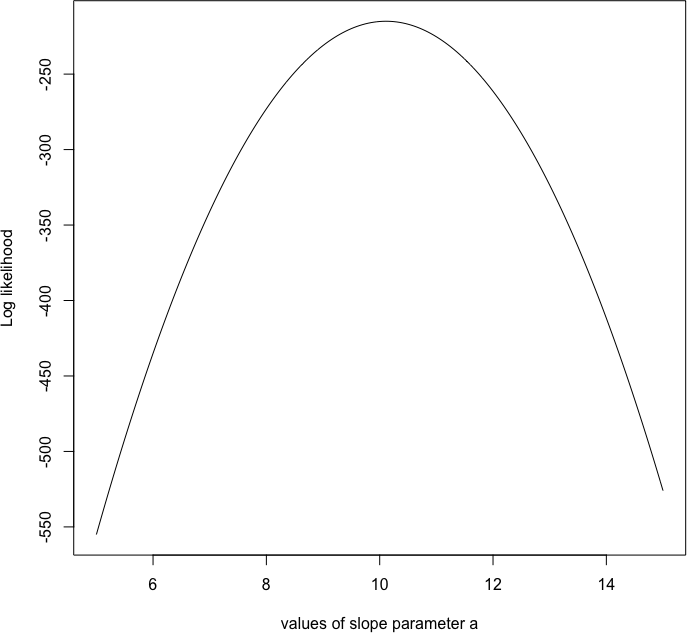
\includegraphics[width=0.9\linewidth]{Images/example9b.png}
\end{center}
\item \textbf{Defining the priors.} In Bayesian analysis, the next step is always required: we have to specify a prior distribution for each of the model parameters. To keep things simple, we will use a uniform distribution for  and normal distributions for all three parameters are used.\footnote{We work with the logarithms of all quantities, so that the likelihood is a sum and not a product as would usually be the case.} 
\begin{lstlisting}
# Prior distribution
prior <- function(param){
    a = param[1]
    b = param[2]
    sd = param[3]
    aprior = dunif(a, min=0, max=2*t.A, log = T)
    bprior = dnorm(b, mean=t.B, sd = 5, log = T)
    sdprior = dunif(sd, min=0, max=2*t.sd, log = T)
    return(aprior+bprior+sdprior)
}
\end{lstlisting}

\item \textbf{The posterior.} The product of prior by likelihood is the actual quantity that MCMC works with (it is not, strictly speaking, the posterior as it is not normalized).

\begin{lstlisting}
posterior <- function(param){
   return (likehd(param) + prior(param))
}
\end{lstlisting}
 
\item \textbf{Applying the MH algorithm.} One of the most frequent applications of MH (as in this example) is sampling from the posterior density in Bayesian statistics.\footnote{The algorithm may be used to sample from any integrable function.} The aim of the algorithm is to jump around in parameter space, but in such a way as to have the probability to land at a point be proportional to the function we sample from (this is usually called the target function). In this case, the target function is the posterior defined previously. \newl This is achieved by 
\begin{enumerate}[noitemsep]
\item starting with a random parameter vector;
\item choosing a new parameter vector near the old value based on some probability density (the proposal function), and 
\item jumping to this new point with a probability $\alpha=\min\{1,g(\text{new})/g(\text{old})\}$, where $g$ is the target.\end{enumerate}
The distribution of the parameter vectors MH visits converges to the target distribution $g$.

\begin{lstlisting}
######## MH ################
proposalfunction <- function(param){
    return(rnorm(3,mean = param, sd= c(0.1,0.5,0.3)))
}
 
run_metropolis_MCMC <- function(startvalue, iterations){
    chain = array(dim = c(iterations+1,3))
    chain[1,] = startvalue
    for (i in 1:iterations){
        proposal = proposalfunction(chain[i,])
         
        probab = exP(posterior(proposal) - posterior(chain[i,]))
        if (runif(1) < probab){
            chain[i+1,] = proposal
        }else{
            chain[i+1,] = chain[i,]
        }
    }
    return(chain)
}
 
startvalue = c(4,0,10)
chain = run_metropolis_MCMC(startvalue, 10000)
 
burnIn = 5000
acceptance = 1-mean(duplicated(chain[-(1:burnIn),]))
\end{lstlisting}
The first steps of the algorithm may be biased by the initialization process; they are usually discarded for the analysis (this is referred to as the \textbf{burn-in time}). \newpage\noindent An interesting output to study is the acceptance rate: how often was a proposal rejected by the MH acceptance criterion? The acceptance rate can be influenced by the proposal function: generally, the nearer the proposal is to the latest value, the larger the acceptance rate. \par Very high acceptance rates, however, are usually not beneficial, as this implies that the algorithms is ``staying'' in the same neighbourhood or point, which results in sub-optimal probing of the parameter space (there is very litte \textbf{mixing}). Acceptance rates between 20\% and 30\% are considered optimal for typical applications \cite{BDA_N11}.\newl
Finally, we can plot the results. 
\begin{lstlisting}

### Summary: #######################
 par(mfrow = c(2,3))
hist(chain[-(1:burnIn),1],nclass=30, , main="Posterior of a", xlab="True value = red line" )
abline(v = mean(chain[-(1:burnIn),1]))
abline(v = t.A, col="red" )
hist(chain[-(1:burnIn),2],nclass=30, main="Posterior of b", xlab="True value = red line")
abline(v = mean(chain[-(1:burnIn),2]))
abline(v = t.B, col="red" )
hist(chain[-(1:burnIn),3],nclass=30, main="Posterior of sd", xlab="True value = red line")
abline(v = mean(chain[-(1:burnIn),3]) )
abline(v = t.sd, col="red" )
plot(chain[-(1:burnIn),1], type = "l", xlab="True value = red line" , main = "Chain values of a", )
abline(h = t.A, col="red" )
plot(chain[-(1:burnIn),2], type = "l", xlab="True value = red line" , main = "Chain values of b", )
abline(h = t.B, col="red" )
plot(chain[-(1:burnIn),3], type = "l", xlab="True value = red line" , main = "Chain values of sd", )
abline(h = t.sd, col="red" )
 
# for comparison:
summary(lm(y~x))

\end{lstlisting}
The resulting plots should look something like those seen in the column on the right: the upper row shows posterior estimates for the slope $a$, intercept $(b)$ and standard deviation of the error ($sd$); the lower row shows the Markov Chain of parameter values. We retrieve (more or less) the original parameters that were used to create the data, and there is a certain area around the highest posterior values that also show some support by the data, which is the Bayesian equivalent of confidence intervals.\newpage\noindent
\begin{center}
		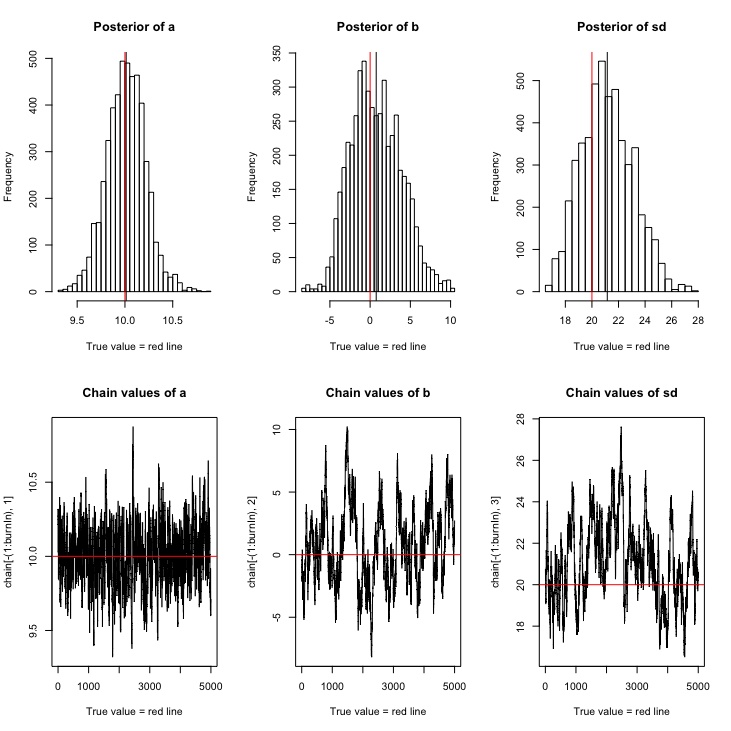
\includegraphics[width=0.9\linewidth]{Images/example9c.png}
\end{center}
The posterior distributions above are \textbf{marginal distributions}, the joint distributions are shown below. 
\begin{center}
		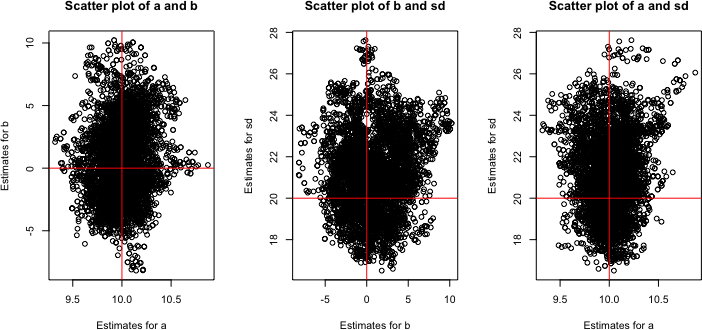
\includegraphics[width=0.9\linewidth]{Images/example9d.png}
\end{center}
By way of comparison, the \texttt{lm()} function in R yields the following estimates: $a$ -- 9.9880 (se: 0.2092), $b$ -- 0.5840 (se: 3.0185), and $sd$ -- 21.34 (48 d.f.).
\end{Example}

\subsection*{Exercises}
\begin{Exercise}
\label{ex4.2.1}
A group of adults are doing a simple learning experiment: when they see the two words ``radio'' and ``ocean'' appear simultaneously on a computer screen, they are asked to press the F key on the keyboard; whenever the words ``radio'' and ``mountain'' appear on the screen, they are asked to press the J key.  After several practice repetitions, two new tasks are introduced: in the first, the word ``radio'' appears by itself and the participants are asked to provide the best response (F or J) based on what they learned before; in the second, the words ``ocean'' and ``mountain'' appear simultaneously and the participants are once again asked to provide the best response. This is repeated with 50 people. The data shows that, for the first test, 40 participants answered with F and 10 with J; while for the second test, 15 responded with F and 35 with J. Are people biased toward F or toward J for either of the two tests? To answer this question, assume a uniform prior, and use a 95\% HDI to decide which biases can be declared to be credible.
\end{Exercise}

%----------------------------------------------------------------------------------------
%----------------Uncertainty-------------------------------------------------------------
%----------------------------------------------------------------------------------------

